
\section{Motivations}
\label{repl:sec:motivations}

Cette section met en évidence les dangers liés à l'utilisation des approches
structures de données répliquées sans résolution de conflits conçues pour les
séquences et n'utilisant pas de pierre tombales. Tout d'abord, des traces
réelles issues de Wikipédia sont employées. Ensuite, des documents artificiels
sont créés de manière à accentuer les comportements des stratégies d'allocation
examinées. Enfin, le problème scientifique est exposé.

\subsection{Traces réelles}

\begin{figure*}
  \centering
  \subfloat[Document Wikipédia principalement édité en fin]
  [\label{repl:img:motivationsA}Document Wikipédia de très grande
  taille principalement édité en fin.]
  {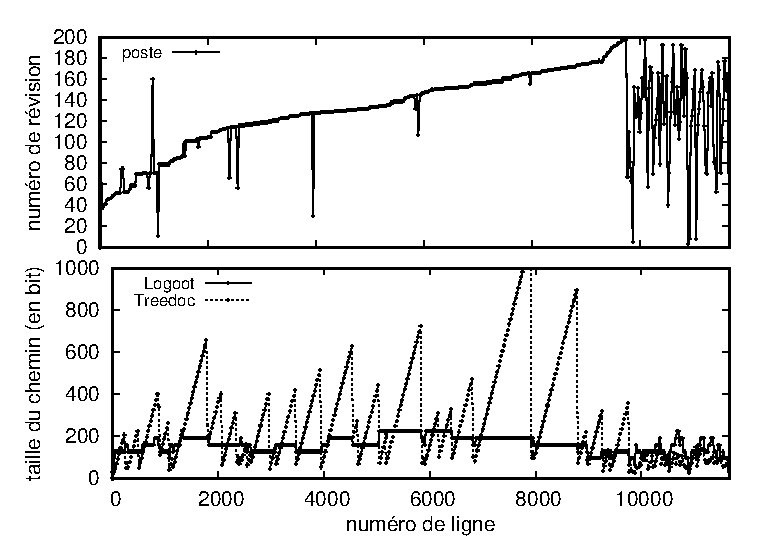
\includegraphics[width=0.8\textwidth]{img/lseq/motivationposte.eps}}
  \hspace{10pt}
  \subfloat[Document Wikipédia principalement édité au début]
  [\label{repl:img:motivationsB}Document Wikipédia de petite taille
  principalement édité au début.]
  {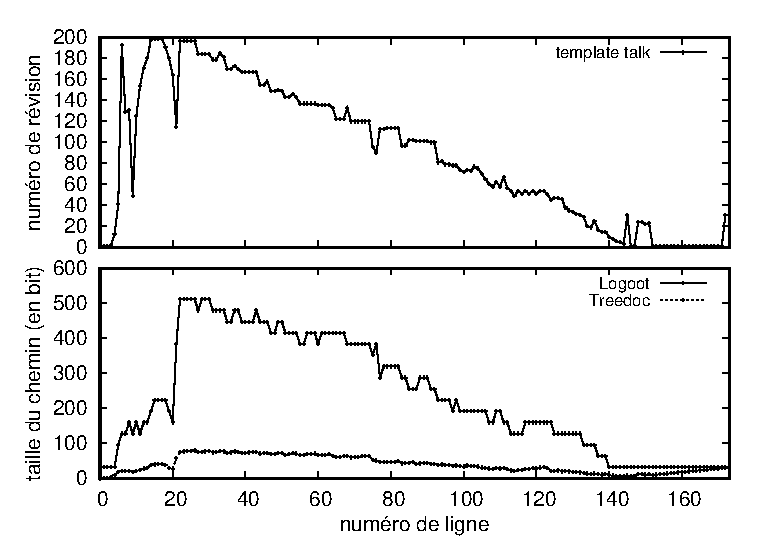
\includegraphics[width=0.8\textwidth]{img/lseq/motivationtemplatetalk.eps}}
  \caption[Taille du chemin alloué pour chaque ligne dans Wikipédia]
  {\label{repl:img:motivations} Taille du chemin alloué pour chaque ligne du
    document. L'axe des abscisses montre le numéro de la ligne concernée. L'axe
    des ordonnées de la partie haute de la figure montre l'âge de la
    ligne. L'axe des ordonnées de la partie basse de la figure montre la taille
    binaire du chemin alloué.}
\end{figure*}

L'encyclopédie Wikipédia~\cite{wikipedia} répertorie des millions d'articles
écrits collaborativement par sa communauté. Un utilisateur, enregistré ou non,
peut lire un article, et s'il le souhaite, en modifier le contenu. Lorsque ses
modifications sont achevées, il les soumet à Wikipédia. Deux issues possibles :
\begin{inparaenum}[(i)]
\item La contribution est acceptée et sera visible de tous ou
\item la contribution est rejetée car un autre utilisateur a effectué une
  modification en concurrence et l'a soumise en premier. Il faut alors réviser
  la version rejetée afin de l'adapter à la version la plus à jour avant de la
  soumettre à nouveau, si nécessaire.
\end{inparaenum}
Wikipédia garde l'historique des modifications apportées à tous les articles
depuis leur création. Nous sommes alors à même de rejouer les éditions --
nommées révision -- dans l'ordre où elles ont été effectuées. Toutefois, la
concurrence qui pourrait exister dans une édition en temps réelle est effacée
par le processus d'édition même. D'autre part, la granularité est fixée à la
ligne. En cela, les simulations sur corpus Wikipédia diffèrent légèrement de la
réalité.

\paragraph{Objectif :} Montrer que ni Logoot ni Treedoc ne parviennent pas à
fournir des identifiants dont la taille soit satisfaisante quel que soit le
document créé grâce à des traces réelles.

\paragraph{Description :} Logoot est configuré avec une base $2^{32}$. Treedoc
est configuré pour utiliser sa méthode originelle -- son autre heuristique
revenant plus ou moins à la stratégie de Logoot. Les documents considérés sont
des articles extraits de Wikipédia et rejoués sur 200 révisions. L'un des
articles atteint jusqu'à 10k lignes principalement ajoutées en fin
d'article\footnote{\scriptsize\url{https://fr.wikipedia.org/wiki/Liste_des_bureaux_de_poste_français_classés_par_oblitération_Petits_Chiffres}}. L'autre
article atteint seulement 200 lignes mais est principalement édité en
tête\footnote{\scriptsize\url{https://en.wikipedia.org/wiki/Template_talk:Did_you_know}}.

\paragraph{Résultat :} Les figures~\ref{repl:img:motivationsA}
et~\ref{repl:img:motivationsB} montrent la taille de l'identifiant associé à
chaque ligne. Nous observons que Treedoc possède des chemins qui augmentent très
vite quel que soit le type d'édition. Lorsque le nombre d'insertions successives
est très grand (cf. figure~\ref{repl:img:motivationsA}) les chemins atteignent
des tailles prohibitives. Dans ce cas, Logoot se comporte mieux. En revanche,
dans le cadre de l'édition en tête, Logoot alloue des chemins dont la taille
augmente extrêmement rapidement. Pour recouvrer de bonnes performances,
l'exécution d'un protocole de relocalisation des chemins devient nécessaire.

\paragraph{Explication :} Dans les deux types d'édition, Treedoc et Logoot
allouent des identifiants dont la complexité est linéaire. Ainsi, plus les
insertions se succèdent, plus l'arbre est déséquilibré, plus la taille du chemin
augmente. Cependant, comme l'arité des chemins Treedoc est binaire
($\mathcal{P}\in \mathbb{N}_{<2}.\mathbb{N}_{<2}\ldots\mathbb{N}_{<2}$), cela
lui permet de conserver des chemins plus petits que ceux de Logoot dans le cadre
du document édité en tête. D'un autre coté, Logoot a conçu sa stratégie pour
l'édition en fin. Dès lors, si le comportement suit cette hypothèse, les
identifiants grossissent par paliers. Linéairement certes, mais lentement. Dans
le cas contraire, les identifiants grimpent très rapidement (cela serait le cas
avec la seconde heuristique de Treedoc).

\subsection{Documents artificiels}


\begin{figure}
  \begin{center}
    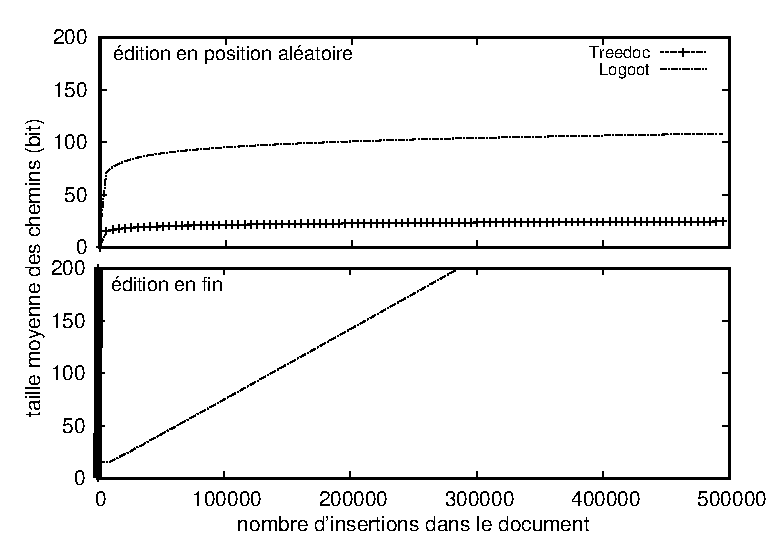
\includegraphics[width=0.8\textwidth]{img/lseq/motivationartificial.eps}
    \caption[Taille moyenne des chemins sur des documents artificiels]
    {\label{repl:img:motivationartificial}Taille moyenne des chemins
      allouées en fonction du nombre d'insertions successives dans le
      document. L'axe des abscisses montre le nombre d'insertions dans le
      documents. L'axe des ordonnées montre la taille moyenne de la
      représentation binaire des chemins alloués.}
  \end{center}
\end{figure}

\paragraph{Objectif :} Montrer la progression de la taille des identifiants
allouées par les fonctions d'allocation Logoot et Treedoc sur des documents
artificiels.

\paragraph{Description :} Deux types de documents artificiels sont créés. Tout
d'abord, un premier document est créé grâce à des insertions à des positions
aléatoires dans la séquence. Le second document est créé grâce à des insertions
successives en fin de document. La fonction d'allocation des chemins de Logoot
est spécifiquement conçue pour gérer ce dernier type d'édition. La taille
moyenne des chemins composant les identifiants est mesurée à chaque nouvelle
insertion. Le document atteint 500k caractères.

\paragraph{Résultat :} La figure~\ref{repl:img:motivationartificial} montre les
résultats de cette simulation. La partie du haut montre les résultats du
document édité à des positions aléatoires. La partie du bas montre les résultats
du document édité à la fin. Nous observons que l'édition à des positions
aléatoires entraîne une génération de chemins dont la taille est logarithmique,
que ce soit pour Logoot ou pour Treedoc. Treedoc est meilleur que Logoot dans ce
cas. Nous observons aussi que l'édition en fin est catastrophique pour Treedoc
(la courbe est superposée à l'axe des ordonnées). De son coté, Logoot alloue des
chemins dont la taille augmente moins rapidement. Malgré cela, la croissance
reste linéaire. À terme, l'exécution d'un protocole de relocalisation des
chemins devient nécessaire pour recouvrir de bonnes performances.

\paragraph{Explication :} Les fonctions d'allocations Logoot et Treedoc
utilisent une structure d'arbres pour allouer le chemin associé à chaque
caractère. Dans le cadre de l'édition aléatoire, l'arbre reste équilibré au
cours des insertions. Les branches les plus basses se remplissent au maximum de
leur capacité. Par conséquent, les identifiants alloués par Treedoc et Logoot
croissent logarithmiquement par rapport au nombre d'insertion. L'arité de
l'arbre de Treedoc étant inférieure à l'arité de l'arbre de Logoot, Treedoc
propose de meilleures performances. Dans le cadre de l'édition en fin, chaque
nouvelle insertion dans Treedoc ajoute un bit au chemin généré. La croissance
est linéaire comparée au nombre d'insertions dans la séquence et extrêmement
rapide. La fonction d'allocation de Logoot est conçue pour gérer ce type
d'édition. Une branche par niveau de l'arbre se trouve bien remplie
d'éléments. Toutefois, le nombre d'éléments accueillis par chaque branche reste
constant, d'où la croissance linéaire de la taille des chemins générés.

\subsection{Définition du problème}

Pour éviter l'exécution d'un protocole de relocalisation des identifiants au
coût prohibitivement élevé, une fonction d'allocation d'identifiants doit être
sous-linéaire par rapport au nombre d'insertions dans le document, quel que soit
le comportement d'édition. La difficulté réside dans le fait qu'aucune
connaissance concernant l'édition n'est disponible. En particulier, ni le nombre
ni la position des insertions ne sont connus par avance.

La section suivante présente une fonction d'allocation d'identifiants dont la
taille, dans le contexte de l'édition collaborative, reste bornée
polylogarithmiquement par rapport au nombre d'insertions effectuées dans la
séquence.

%%% Local Variables:
%%% mode: latex
%%% TeX-master: "../../paper"
%%% End:
